\documentclass[11pt,draft]{cmuthesis}
%> ---------------------------------------------------------------------------------------------------------------
%> Line spacing. Neither EPP nor College of Engineering mandates either single- or double-spacing.
%> The default is to use single-spacing. If you want to use one-and-a-half or double-spacing,
%> uncomment ONE the following lines.
%\onehalfspacing
%\doublespacing

%> ---------------------------------------------------------------------------------------------------------------
%> Put here all those things that are common to the whole thesis. It makes sense
%> to put names that may change, or some numbers that you repeat many times but
%> are amenable to change; e.g., the number of participants in your studies.
\newcommand{\TotalParticipantsStudyOne}[0]{573}
\newcommand{\TotalParticipantsStudyTwo}[0]{982}


\begin{document}
%> First pages. Do not modify.
\frontmatter
\pagestyle{plain}
%> ------------------------------------------------------------------------------
%> This file contains most of the definitions you will need to put together
%> your thesis. All requirements were taken from the sources below:
%> http://www.cit.cmu.edu/current_students/graduates/thesis_dissertation_policies.html
%> https://www.epp.cmu.edu/graduate/thesis_format_guide.html
%> ------------------------------------------------------------------------------
\frontmatter\pagestyle{plain}

%> Your title goes here.
\title{Your Title Here: A Journey to the Deeps of Knowledge}

%> Your own name goes here.
\author{John Doe}

%> Put your previous degrees here.
\bsdegree{Mechanical Engineering, West Knot University}
\msdegree{Mechanical Engineering, Carnegie Mellon University}

%> Put the month you will be graduating here, NOT the month in which you
%> actually finished the thesis. The only admissible months here are May,
%> August and December.
\Month{December}

%> Year in which you graduated (or plan to graduate).
\Year{2018}

%> Copyright notice. This may be whatever you want. My personal choice is to
%> make it as widely accessible as possible :)
\permission{\textit{Some rights reserved.} Except where indicated, this work
is licensed under a Creative Commons Attribution 3.0 United States License. 
Please see \smallurl{http://creativecommons.org/licenses/by/3.0/us/} for
details.}

%> Keywords.
\keywords{artificial intelligence, sustainaible engineering, green design,
cyber-security, carbon sequestration.}
\maketitle

%> ------------------------------------------------------------------------------
%> Abstract. Mandatory and very important. Keep it under 350 words.
%> ------------------------------------------------------------------------------
\begin{abstract}
Lorem ipsum dolor sit amet, consectetur adipiscing elit. Fusce enim nunc,
viverra vitae placerat nec, lacinia at augue. Sed varius ullamcorper dolor
id suscipit. Suspendisse posuere augue vitae sapien faucibus mattis et non
ante. Pellentesque sed mauris sit amet neque fringilla scelerisque in vitae
quam. Cras congue adipiscing nisi, ac aliquam nulla porta in. Nam id nisi
ornare, accumsan sapien et, consequat nisi. Donec egestas risus a massa
mollis pellentesque. Sed in pretium tortor, in euismod nisl. Phasellus
lacinia orci eu lacus posuere, ut imperdiet tortor aliquam. Morbi at
vestibulum mauris. Quisque tristique, nunc sit amet suscipit suscipit, erat
lacus consectetur lorem, sed luctus ante felis in magna. Donec vitae metus
quis ante feugiat varius in vitae ligula.

Sed auctor, elit quis venenatis semper, velit purus mattis orci, vitae
pellentesque mauris leo ut sapien. Ut aliquet libero diam, sed congue erat
suscipit non. Curabitur facilisis nibh sodales purus varius interdum. Cum
sociis natoque penatibus et magnis dis parturient montes, nascetur ridiculus
mus. Sed sed faucibus lorem. Suspendisse potenti. Duis sagittis sagittis
lobortis. Vestibulum nec magna sed urna ultrices dignissim. Curabitur et
justo mauris.
\end{abstract}

%> ------------------------------------------------------------------------------
%> Dedication. Optional. This is whatever you want.
%> ------------------------------------------------------------------------------
\begin{dedication}
Nullam sit amet diam felis. Aenean pulvinar cursus diam rhoncus bibendum.
Suspendisse sit amet porttitor sem. Suspendisse euismod metus ut ligula
interdum malesuada. Sed hendrerit est et turpis imperdiet, commodo
vestibulum enim eleifend. Etiam tellus sapien, volutpat ac leo eu, hendrerit
vestibulum metus. Donec sit amet suscipit lectus. Nam at nunc sodales turpis
rhoncus ullamcorper in eu risus. Proin nec nulla eu ipsum tincidunt
fermentum nec a ligula. Etiam imperdiet, ligula eget fermentum pellentesque,
tortor ligula pulvinar ante, ut aliquet ante nisi eget nulla. Class aptent
taciti sociosqu ad litora torquent per conubia nostra, per inceptos
himenaeos. Cras quis condimentum sem. Aliquam rhoncus, lacus id fringilla
elementum, ligula lectus vestibulum ipsum, sed pellentesque orci felis non
sapien. Aenean dolor lorem, pharetra adipiscing metus nec, eleifend
elementum ante. Nulla scelerisque interdum sem faucibus fermentum. In
posuere tempus lectus, ac gravida justo fringilla nec.
\end{dedication}


%> ------------------------------------------------------------------------------
%> Acknowledgements. Mandatory. At the very least you should acknowledge
%> your committee and your funding sources.
%> ------------------------------------------------------------------------------
\begin{acknowledgments}
Lorem ipsum dolor sit amet, consectetur adipiscing elit. Fusce enim nunc,
viverra vitae placerat nec, lacinia at augue. Sed varius ullamcorper dolor
id suscipit. Suspendisse posuere augue vitae sapien faucibus mattis et non
ante.

Pellentesque sed mauris sit amet neque fringilla scelerisque in vitae
quam. Cras congue adipiscing nisi, ac aliquam nulla porta in. Nam id nisi
ornare, accumsan sapien et, consequat nisi. Donec egestas risus a massa
mollis pellentesque.

Sed in pretium tortor, in euismod nisl. Phasellus
lacinia orci eu lacus posuere, ut imperdiet tortor aliquam. Morbi at
vestibulum mauris.

Quisque tristique, nunc sit amet suscipit suscipit, erat
lacus consectetur lorem, sed luctus ante felis in magna. Donec vitae metus
quis ante feugiat varius in vitae ligula.
\end{acknowledgments}

%> ------------------------------------------------------------------------------
%> Table of contents, List of figures, etc. Do not modify.
%> ------------------------------------------------------------------------------

\tableofcontents
\listoffigures
\listoftables
\mainmatter

%> Configuration of the headers
\pagestyle{fancy}
\lhead[\footnotesize\emph{\chaptername\ \thechapter. \leftmark}]{}
\rhead[]{\footnotesize\emph{\thesection. \rightmark}}

\tableofcontents
\listoffigures
\listoftables
\mainmatter

%> Configuration of the headers
\pagestyle{fancy}
\lhead[\footnotesize\emph{\chaptername\ \thechapter. \leftmark}]{}
\rhead[]{\footnotesize\emph{\thesection. \rightmark}}


%> Content. This section contains references to the chapters in your thesis.
%> Modify as you please.
\chapter{Introduction}
\label{chp:intro}

Lorem ipsum dolor sit amet, consectetur adipiscing elit. Fusce enim nunc,
viverra vitae placerat nec, lacinia at augue.  Sed varius ullamcorper dolor
id suscipit.  Suspendisse posuere augue vitae sapien faucibus mattis et non
ante \cite{Bahr2011}.  Pellentesque sed mauris sit amet neque fringilla
scelerisque in vitae quam.  Cras congue adipiscing nisi, ac aliquam nulla
porta in \cite{Witte92}.  Nam id nisi ornare, accumsan sapien et, consequat
nisi.  Donec egestas risus a massa mollis pellentesque.  Sed in pretium
tortor, in euismod nisl.  Phasellus lacinia orci eu lacus posuere, ut
imperdiet tortor aliquam.  Morbi at vestibulum mauris.  Quisque tristique,
nunc sit amet suscipit suscipit, erat lacus consectetur lorem, sed luctus
ante felis in magna \cite{Morgan2002}.  Donec vitae metus quis ante feugiat varius in vitae
ligula.

\begin{table}
\centering
\begin{tabular}{|c|c|l|} \hline
Non-English or Math&Frequency&Comments\\ \hline
\O & 1 in 1,000& For Swedish names\\ \hline
$\pi$ & 1 in 5& Common in math\\ \hline
\$ & 4 in 5 & Used in business\\ \hline
$\Psi^2_1$ & 1 in 40,000& Unexplained usage\\
\hline\end{tabular}
\caption{Frequency of Special Characters}
\label{tab:specialchars}
\end{table}

Sed auctor, elit quis venenatis semper \cite{Anderson2005}, velit purus
mattis orci, vitae pellentesque mauris leo ut sapien.  Ut aliquet libero
diam, sed congue erat suscipit non.  Curabitur facilisis nibh sodales purus
varius interdum.  Cum sociis natoque penatibus et magnis dis parturient
montes, nascetur ridiculus mus.  Sed sed faucibus lorem.  Suspendisse
potenti.  Duis sagittis sagittis lobortis.  Vestibulum nec magna sed urna
ultrices dignissim.  Curabitur et justo mauris.

Nulla varius diam turpis, nec consequat dolor semper ut. Suspendisse
pellentesque, dui sed vulputate auctor, dolor magna aliquet lorem, sed
pulvinar nisl turpis sed metus. Ut massa quam, cursus et mollis quis, cursus
vel justo. Interdum et malesuada fames ac ante ipsum primis in faucibus.
Proin sodales fringilla justo \cite{Morgan2002}, quis bibendum felis ullamcorper in.
Suspendisse congue, quam id malesuada dignissim, purus dui hendrerit enim,
et facilisis odio enim eu est. Donec at turpis quam. Ut blandit diam ac
sapien dignissim, non porttitor diam dictum. Donec eget massa gravida,
iaculis lorem eleifend, pellentesque quam. Nunc ligula mauris, consectetur
at fringilla eget, auctor eu purus. Proin eu auctor elit. Etiam tempor
malesuada consequat. Mauris imperdiet purus ac erat viverra, iaculis laoreet
ligula molestie. Nunc ac justo augue \cite{Morgan2002}. Morbi lorem nunc, condimentum non
lectus et, tempus accumsan quam. Vestibulum velit elit, mollis quis metus
at, tempor consequat massa.

\section{Research questions}

\begin{quote}\itshape In this thesis, I make the following contributions:
Lorem ipsum dolor sit amet, consectetur adipiscing elit; fusce enim nunc,
viverra vitae placerat nec, lacinia at augue; and sed varius ullamcorper dolor
id suscipit.\end{quote}

Sed auctor, elit quis venenatis semper \cite{Anderson2005}, velit purus
mattis orci, vitae pellentesque mauris leo ut sapien.  Ut aliquet libero
diam, sed congue erat suscipit non.  Curabitur facilisis nibh sodales purus
varius interdum.  Cum sociis natoque penatibus et magnis dis parturient
montes, nascetur ridiculus mus \cite{Morgan2002}.  Sed sed faucibus lorem.  Suspendisse
potenti.  Duis sagittis sagittis lobortis.  Vestibulum nec magna sed urna
ultrices dignissim.  Curabitur et justo mauris.

\begin{enumerate}

\item Nulla varius diam turpis, nec consequat dolor semper ut. Suspendisse
pellentesque, dui sed vulputate auctor, dolor magna aliquet lorem, sed
pulvinar nisl turpis sed metus?  (Chapter \ref{chp:studyone})

\item Ut massa quam, cursus et mollis quis, cursus vel justo.  Interdum et
malesuada fames ac ante ipsum primis in faucibus.  Proin sodales fringilla
justo, quis bibendum felis ullamcorper in.  Suspendisse congue, quam id
malesuada dignissim, purus dui hendrerit enim, et facilisis odio enim eu
est?  (Chapter \ref{chp:studytwo})

\item Donec at turpis quam. Ut blandit diam ac
sapien dignissim, non porttitor diam dictum. Donec eget massa gravida,
iaculis lorem eleifend, pellentesque quam. Nunc ligula mauris, consectetur
at fringilla eget, auctor eu purus. Proin eu auctor elit? (Chapter
\ref{chp:studythree})

\end{enumerate}

\section{Thesis overview}

In Chapter \ref{chp:relatedwork}, nulla varius diam turpis, nec consequat
dolor semper ut.  Suspendisse pellentesque, dui sed vulputate auctor, dolor
magna aliquet lorem, sed pulvinar nisl turpis sed metus.  Ut massa quam,
cursus et mollis quis, cursus vel justo.  Interdum et malesuada fames ac
ante ipsum primis in faucibus.

In Chapter \ref{chp:studyone}, proin sodales fringilla justo, quis bibendum
felis ullamcorper in.  Suspendisse congue, quam id malesuada dignissim,
purus dui hendrerit enim, et facilisis odio enim eu est.  Donec at turpis
quam.  Ut blandit diam ac sapien dignissim, non porttitor diam dictum.

In Chapter \ref{chp:studytwo}, donec eget massa gravida, iaculis lorem
eleifend, pellentesque quam.  Nunc ligula mauris, consectetur at fringilla
eget, auctor eu purus.  Proin eu auctor elit.  Etiam tempor malesuada
consequat.

In Chapter \ref{chp:studythree}, mauris imperdiet purus ac erat viverra,
iaculis laoreet ligula molestie.  Nunc ac justo augue.  Morbi lorem nunc,
condimentum non lectus et, tempus accumsan quam.  Vestibulum velit elit,
mollis quis metus at, tempor consequat massa.

Finally, in Chapter \ref{chp:conclusions}, sed auctor, elit quis venenatis
semper \cite{Anderson2005}, velit purus mattis orci, vitae pellentesque
mauris leo ut sapien.  Ut aliquet libero diam, sed congue erat suscipit non. 
Curabitur facilisis nibh sodales purus varius interdum.  Cum sociis natoque
penatibus et magnis dis parturient montes, nascetur ridiculus mus.  Sed sed
faucibus lorem.  Suspendisse potenti.  Duis sagittis sagittis lobortis. 
Vestibulum nec magna sed urna ultrices dignissim.  Curabitur et justo
mauris.
\chapter{Background and Related work}
\label{chp:relatedwork}

Lorem ipsum dolor sit amet, consectetur adipiscing elit. Fusce enim nunc,
viverra vitae placerat nec, lacinia at augue. Sed varius ullamcorper dolor
id suscipit. Suspendisse posuere augue vitae sapien faucibus mattis et non
ante. Pellentesque sed mauris sit amet neque fringilla scelerisque in vitae
quam. Cras congue adipiscing nisi, ac aliquam nulla porta in. Nam id nisi
ornare, accumsan sapien et, consequat nisi. Donec egestas risus a massa
mollis pellentesque. \eddelete{Sed in pretium tortor, in euismod nisl. Phasellus
lacinia orci eu lacus posuere, ut imperdiet tortor aliquam. Morbi at
vestibulum mauris.} Quisque tristique, nunc sit amet suscipit suscipit, erat
lacus consectetur lorem, sed luctus ante felis in magna. Donec vitae metus
quis ante feugiat varius in vitae ligula.

\section{Background}
Sed auctor, elit quis venenatis semper, velit purus mattis orci, vitae
pellentesque mauris leo ut sapien. Ut aliquet libero diam, sed congue erat
suscipit non. Curabitur facilisis nibh sodales purus varius interdum. Cum
sociis natoque penatibus et magnis dis parturient montes, nascetur ridiculus
mus. Sed sed faucibus lorem. Suspendisse potenti. Duis sagittis sagittis
lobortis. Vestibulum nec magna sed urna ultrices dignissim. Curabitur et
justo mauris. \comment{No, wait! You got it all wrong! Change this back to
what it was!}

\section{Something else}
Nulla varius diam turpis, nec consequat dolor semper ut. Suspendisse
pellentesque, dui sed vulputate auctor, dolor magna aliquet lorem, sed
pulvinar nisl turpis sed metus. \comment{You should also add the discussion
about Roth et al.\ here} Ut massa quam, cursus et mollis quis, cursus
vel justo. Interdum et malesuada fames ac ante ipsum primis in faucibus.
Proin sodales fringilla justo, quis bibendum felis ullamcorper in.
Suspendisse congue, quam id malesuada dignissim, purus dui hendrerit enim,
et facilisis odio enim eu est. Donec at turpis quam. Ut blandit diam ac
sapien dignissim, non porttitor diam dictum. \comment{This may change in any
minute, so don't hold on to it.} Donec eget massa gravida,
iaculis lorem eleifend, pellentesque quam. Nunc ligula mauris, consectetur
at fringilla eget, auctor eu purus. Proin eu auctor elit. Etiam tempor
malesuada consequat. Mauris imperdiet purus ac erat viverra, iaculis laoreet
ligula molestie. Nunc ac justo augue. \edadd{Morbi lorem nunc, condimentum non
lectus et, tempus accumsan quam.} Vestibulum velit elit, mollis quis metus
at, tempor consequat massa.

\section{Other findings}
\eddelete{Donec egestas risus a massa
mollis pellentesque. Sed in pretium tortor, in euismod nisl. Phasellus
lacinia orci eu lacus posuere, ut imperdiet tortor aliquam. Morbi at
vestibulum mauris. Quisque tristique, nunc sit amet suscipit suscipit, erat
lacus consectetur lorem, sed luctus ante felis in magna. Donec vitae metus
quis ante feugiat varius in vitae ligula.}

Nulla varius diam turpis, nec consequat dolor semper ut. Suspendisse
pellentesque, dui sed vulputate auctor, dolor magna aliquet lorem, sed
pulvinar nisl turpis sed metus. Ut massa quam, cursus et mollis quis, cursus
vel justo. Interdum et malesuada fames ac ante ipsum primis in faucibus.
Proin sodales fringilla justo, quis bibendum felis ullamcorper in.
Suspendisse congue, quam id malesuada dignissim, purus dui hendrerit enim,
et facilisis odio enim eu est. Donec at turpis quam. Ut blandit diam ac
sapien dignissim, non porttitor diam dictum. Donec eget massa gravida,
iaculis lorem eleifend, pellentesque quam. Nunc ligula mauris, consectetur
at fringilla eget, auctor eu purus. Proin eu auctor elit. Etiam tempor
malesuada consequat. Mauris imperdiet purus ac erat viverra, iaculis laoreet
ligula molestie. Nunc ac justo augue. Morbi lorem nunc, condimentum non
lectus et, tempus accumsan quam. Vestibulum velit elit, mollis quis metus
at, tempor consequat massa.

\chapter[Exploratory study on Lorem Ipsum]{Exploratory study on Lorem Ipsum:
where everything began}
\label{chp:studyone}
\blindfootnote{This chapter is based on Akhawe and Felt, 2013 \cite{AkhaweEtFelt2013}.}

Lorem ipsum dolor sit amet, consectetur adipiscing elit. Fusce enim nunc,
viverra vitae placerat nec, lacinia at augue.  Sed varius ullamcorper dolor
id suscipit.  Suspendisse posuere augue vitae sapien faucibus mattis et non
ante.  Pellentesque sed mauris sit amet neque fringilla scelerisque in vitae
quam.  Cras congue adipiscing nisi, ac aliquam nulla porta in.  Nam id nisi
ornare, accumsan sapien et, consequat nisi.  Donec egestas risus a massa
mollis pellentesque.  Sed in pretium tortor, in euismod nisl.  Phasellus
lacinia orci eu lacus posuere, ut imperdiet tortor aliquam.  Morbi at
vestibulum mauris.  Quisque tristique, nunc sit amet suscipit suscipit, erat
lacus consectetur lorem, sed luctus ante felis in magna.  Donec vitae metus
quis ante feugiat varius in vitae ligula.

\section{Introduction} \label{sec:studyone:intro}

Sed auctor, elit quis venenatis semper, velit purus mattis orci, vitae
pellentesque mauris leo ut sapien.  Ut aliquet libero diam, sed congue erat
suscipit non.  Curabitur facilisis nibh sodales purus varius interdum.  Cum
sociis natoque penatibus et magnis dis parturient montes, nascetur ridiculus
mus.  Sed sed faucibus lorem.  Suspendisse potenti.  Duis sagittis sagittis
lobortis.  Vestibulum nec magna sed urna ultrices dignissim.  Curabitur et
justo mauris.

Nulla varius diam turpis, nec consequat dolor semper ut. Suspendisse
pellentesque, dui sed vulputate auctor, dolor magna aliquet lorem, sed
pulvinar nisl turpis sed metus.  Ut massa quam, cursus et mollis quis,
cursus vel justo.  Interdum et malesuada fames ac ante ipsum primis in
faucibus.  Proin sodales fringilla justo, quis bibendum felis ullamcorper
in.  Suspendisse congue, quam id malesuada dignissim, purus dui hendrerit
enim, et facilisis odio enim eu est.  Donec at turpis quam.  Ut blandit diam
ac sapien dignissim, non porttitor diam dictum.  Donec eget massa gravida,
iaculis lorem eleifend, pellentesque quam.  Nunc ligula mauris, consectetur
at fringilla eget, auctor eu purus.  Proin eu auctor elit.  Etiam tempor
malesuada consequat.  Mauris imperdiet purus ac erat viverra, iaculis
laoreet ligula molestie.  Nunc ac justo augue.  Morbi lorem nunc,
condimentum non lectus et, tempus accumsan quam.  Vestibulum velit elit,
mollis quis metus at, tempor consequat massa.

\section{Methods}
\label{sec:studyone:methods}

Nullam sit amet diam felis. Aenean pulvinar cursus diam rhoncus bibendum.
Suspendisse sit amet porttitor sem.  Suspendisse euismod metus ut ligula
interdum malesuada.  Sed hendrerit est et turpis imperdiet, commodo
vestibulum enim eleifend.  Etiam tellus sapien, volutpat ac leo eu,
hendrerit vestibulum metus.  Donec sit amet suscipit lectus.  Nam at nunc
sodales turpis rhoncus ullamcorper in eu risus.  Proin nec nulla eu ipsum
tincidunt fermentum nec a ligula.  Etiam imperdiet, ligula eget fermentum
pellentesque, tortor ligula pulvinar ante, ut aliquet ante nisi eget nulla. 
Class aptent taciti sociosqu ad litora torquent per conubia nostra, per
inceptos himenaeos.  Cras quis condimentum sem.  Aliquam rhoncus, lacus id
fringilla elementum, ligula lectus vestibulum ipsum, sed pellentesque orci
felis non sapien.  Aenean dolor lorem, pharetra adipiscing metus nec,
eleifend elementum ante.  Nulla scelerisque interdum sem faucibus fermentum. 
In posuere tempus lectus, ac gravida justo fringilla nec.

\section{Results}
\label{sec:studyone:results}

Nulla sollicitudin, lorem ac feugiat bibendum (\TotalParticipantsStudyOne{} participants), neque erat ornare nulla, id
mattis nibh velit eget ante.  Duis \TotalParticipantsStudyOne{} participants tincidunt viverra mi, quis malesuada est
convallis id.  Nunc et pulvinar lorem, et tincidunt felis.  Aenean pretium
elit quis leo elementum lacinia.  Proin at sagittis eros.  Etiam sed tortor
id risus viverra dapibus ut eget nunc.  Duis consectetur, nisl ac malesuada
iaculis, libero dolor facilisis risus, quis aliquam arcu augue et libero. 
Phasellus eget feugiat nunc, ac pretium diam.

\section{Discussion}
\label{sec:studyone:discussion}

Nullam sit amet diam felis for a total of \TotalParticipantsStudyOne{} participants. Aenean pulvinar cursus diam rhoncus bibendum.
Suspendisse sit amet porttitor sem.  Suspendisse euismod metus ut ligula
interdum malesuada.  Sed hendrerit est et turpis imperdiet, commodo
vestibulum enim eleifend.  Etiam tellus sapien, volutpat ac leo eu,
hendrerit vestibulum metus.  Donec sit amet suscipit lectus.  Nam at nunc
sodales turpis rhoncus ullamcorper in eu risus.  Proin nec nulla eu ipsum
tincidunt fermentum nec a ligula.  Etiam imperdiet, ligula eget fermentum
pellentesque, tortor ligula pulvinar ante, ut aliquet ante nisi eget nulla. 
Class aptent taciti sociosqu ad litora torquent per conubia nostra, per
inceptos himenaeos.  Cras quis condimentum sem.  Aliquam rhoncus, lacus id
fringilla elementum, ligula lectus vestibulum ipsum, sed pellentesque orci
felis non sapien.  Aenean dolor lorem, pharetra adipiscing metus nec,
eleifend elementum ante.  Nulla scelerisque interdum sem faucibus fermentum. 
In posuere tempus lectus, ac gravida justo fringilla nec.

Nulla sollicitudin, lorem ac feugiat bibendum, neque erat ornare nulla, id
mattis nibh velit eget ante.  Duis tincidunt viverra mi, quis malesuada est
convallis id.  Nunc et pulvinar lorem, et tincidunt felis.  Aenean pretium
elit quis leo elementum lacinia.  Proin at sagittis eros.  Etiam sed tortor
id risus viverra dapibus ut eget nunc.  Duis consectetur, nisl ac malesuada
iaculis, libero dolor facilisis risus, quis aliquam arcu augue et libero. 
Phasellus eget feugiat nunc, ac pretium diam.

\section{Conclusions}
\label{sec:studyone:conclusions}

Nullam sit amet diam felis. Aenean pulvinar cursus diam rhoncus bibendum.
Suspendisse sit amet porttitor sem.  Suspendisse euismod metus ut ligula
interdum malesuada.  Sed hendrerit est et turpis imperdiet, commodo
vestibulum enim eleifend.  Etiam tellus sapien, volutpat ac leo eu,
hendrerit vestibulum metus.  Donec sit amet suscipit lectus.  Nam at nunc
sodales turpis rhoncus ullamcorper in eu risus.  Proin nec nulla eu ipsum
tincidunt fermentum nec a ligula.  Etiam imperdiet, ligula eget fermentum
pellentesque, tortor ligula pulvinar ante, ut aliquet ante nisi eget nulla. 
Class aptent taciti sociosqu ad litora torquent per conubia nostra, per
inceptos himenaeos.  Cras quis condimentum sem.  Aliquam rhoncus, lacus id
fringilla elementum, ligula lectus vestibulum ipsum, sed pellentesque orci
felis non sapien.  Aenean dolor lorem, pharetra adipiscing metus nec,
eleifend elementum ante.  Nulla scelerisque interdum sem faucibus fermentum. 
In posuere tempus lectus, ac gravida justo fringilla nec.

Nulla sollicitudin, lorem ac feugiat bibendum, neque erat ornare nulla, id
mattis nibh velit eget ante.  Duis tincidunt viverra mi, quis malesuada est
convallis id.  Nunc et pulvinar lorem, et tincidunt felis.  Aenean pretium
elit quis leo elementum lacinia.  Proin at sagittis eros.  Etiam sed tortor
id risus viverra dapibus ut eget nunc.  Duis consectetur, nisl ac malesuada
iaculis, libero dolor facilisis risus, quis aliquam arcu augue et libero. 
Phasellus eget feugiat nunc, ac pretium diam.

\chapter[Simple techniques to decrease micro-ruptures]{Water-proof,
thermo-resilient O-Rings: simple techniques to decrease micro-ruptures}
\label{chp:studytwo}
\blindfootnote{This chapter is based on Bahr and Ford, 2013 \cite{Bahr2011}.}

Lorem ipsum dolor sit amet, consectetur adipiscing elit. Fusce enim nunc,
viverra vitae placerat nec, lacinia at augue.  Sed varius ullamcorper dolor
id suscipit.  Suspendisse posuere augue vitae sapien faucibus mattis et non
ante (see Section \ref{sec:studyone:discussion}).  Pellentesque sed mauris
sit amet neque fringilla scelerisque in vitae quam.  Cras congue adipiscing
nisi, ac aliquam nulla porta in.  Nam id nisi ornare, accumsan sapien et,
consequat nisi.  Donec egestas risus a massa mollis pellentesque.  Sed in
pretium tortor, in euismod nisl.  Phasellus lacinia orci eu lacus posuere,
ut imperdiet tortor aliquam.  Morbi at vestibulum mauris.  Quisque
tristique, nunc sit amet suscipit suscipit, erat lacus consectetur lorem,
sed luctus ante felis in magna.  Donec vitae metus quis ante feugiat varius
in vitae ligula.

\section{Introduction}
\label{sec:studytwo:intro}

Sed auctor, elit quis venenatis semper, velit purus mattis orci, vitae
pellentesque mauris leo ut sapien.  Ut aliquet libero diam, sed congue erat
suscipit non.  Curabitur facilisis nibh sodales purus varius interdum.  Cum
sociis natoque penatibus et magnis dis parturient montes, nascetur ridiculus
mus (see Section \ref{sec:studyone:conclusions}).  Sed sed faucibus lorem. 
Suspendisse potenti.  Duis sagittis sagittis lobortis.  Vestibulum nec magna
sed urna ultrices dignissim.  Curabitur et justo mauris.

Nulla varius diam turpis, nec consequat dolor semper ut. Suspendisse
pellentesque, dui sed vulputate auctor, dolor magna aliquet lorem, sed
pulvinar nisl turpis sed metus.  Ut massa quam, cursus et mollis quis,
cursus vel justo.  Interdum et malesuada fames ac ante ipsum primis in
faucibus.  Proin sodales fringilla justo, quis bibendum felis ullamcorper
in.  Suspendisse congue, quam id malesuada dignissim, purus dui hendrerit
enim, et facilisis odio enim eu est.  Donec at turpis quam.  Ut blandit diam
ac sapien dignissim, non porttitor diam dictum.  Donec eget massa gravida,
iaculis lorem eleifend, pellentesque quam.  Nunc ligula mauris, consectetur
at fringilla eget, auctor eu purus.  Proin eu auctor elit.  Etiam tempor
malesuada consequat \cite{Morgan2002}.  Mauris imperdiet purus ac erat
viverra, iaculis laoreet ligula molestie.  Nunc ac justo augue.  Morbi lorem
nunc, condimentum non lectus et, tempus accumsan quam.  Vestibulum velit
elit, mollis quis metus at, tempor consequat massa.

\section{Methods}
\label{sec:studytwo:methods}

Nullam sit amet diam felis. Aenean pulvinar cursus diam rhoncus bibendum.
Suspendisse sit amet porttitor sem.  Suspendisse euismod metus ut ligula
interdum malesuada.  Sed hendrerit est et turpis imperdiet, commodo
vestibulum enim eleifend.  Etiam tellus sapien, volutpat ac leo eu,
hendrerit vestibulum metus.  Donec sit amet suscipit lectus.  Nam at nunc
sodales turpis rhoncus ullamcorper in eu risus.  Proin nec nulla eu ipsum
tincidunt fermentum nec a ligula.  Etiam imperdiet, ligula eget fermentum
pellentesque, tortor ligula pulvinar ante, ut aliquet ante nisi eget nulla. 
Class aptent taciti sociosqu ad litora torquent per conubia nostra, per
inceptos himenaeos.  Cras quis condimentum sem.  Aliquam rhoncus, lacus id
fringilla elementum, ligula lectus vestibulum ipsum, sed pellentesque orci
felis non sapien.  Aenean dolor lorem, pharetra adipiscing metus nec,
eleifend elementum ante.  Nulla scelerisque interdum sem faucibus fermentum. 
In posuere tempus lectus, ac gravida justo fringilla nec.

\section{Results}
\label{sec:studytwo:results}

Nulla sollicitudin, lorem ac feugiat bibendum, neque erat ornare nulla, id
mattis nibh velit eget ante.  Duis tincidunt viverra mi, quis malesuada est
convallis id.  Nunc et pulvinar lorem, et tincidunt felis.  Aenean pretium
elit quis leo elementum lacinia.  Proin at sagittis eros.  Etiam sed tortor
id risus viverra dapibus ut eget nunc.  Duis consectetur, nisl ac malesuada
iaculis, libero dolor facilisis risus, quis aliquam arcu augue et libero. 

\begin{figure}\centering
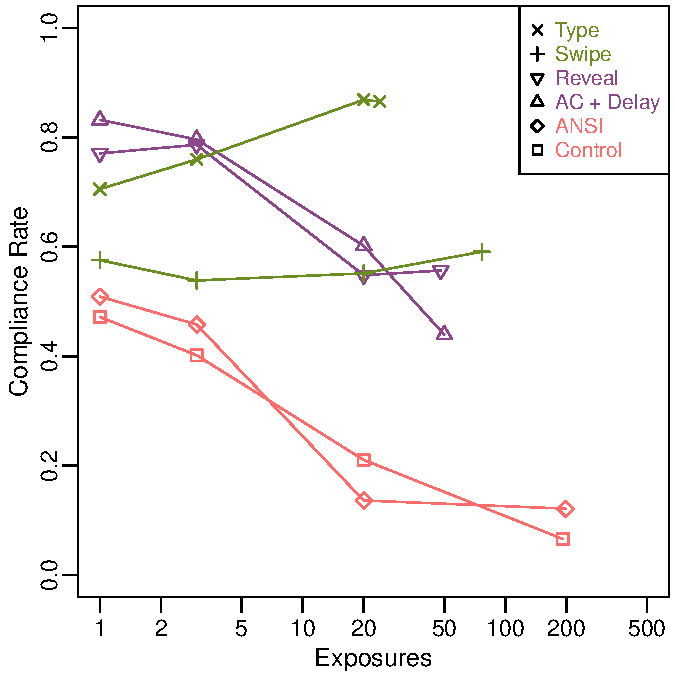
\includegraphics[scale=0.8]{chp-studytwo/images/fig-studytwo-results.pdf}
\caption[
	Aliquam in nibh urna. Maecenas vitae malesuada tellus, sit amet
	interdum metus.  Maecenas enim urna, consequat interdum leo vel,
	egestas mollis enim.
]{
	Aliquam in nibh urna. Maecenas vitae malesuada tellus, sit amet
	interdum metus.  Maecenas enim urna, consequat interdum leo vel,
	egestas mollis enim.  Aenean ut lacinia lacus.  Cum sociis natoque
	penatibus et magnis dis parturient montes, nascetur ridiculus mus. 
	Donec non molestie lacus.  Fusce et neque turpis.  Duis sagittis
	scelerisque ipsum vel pellentesque.  In porta magna lectus, sit amet
	rhoncus dui mollis at.  Suspendisse potenti.  Nulla sagittis lobortis
	neque vel tincidunt.  Etiam eu eros nisi.  Cras eleifend pellentesque
	ipsum, et vehicula neque sodales sit amet.  Pellentesque in lacus
	ipsum.
}
\label{fig:studytwo:results}
\end{figure}


Phasellus eget feugiat nunc, ac pretium diam.

\section{Discussion}
\label{sec:studytwo:discussion}

Nullam sit amet diam felis. Aenean pulvinar cursus diam rhoncus bibendum.
Suspendisse sit amet porttitor sem.  Suspendisse euismod metus ut ligula
interdum malesuada.  Sed hendrerit est et turpis imperdiet, commodo
vestibulum enim eleifend.  Etiam tellus sapien, volutpat ac leo eu,
hendrerit vestibulum metus.  Donec sit amet suscipit lectus.  Nam at nunc
sodales turpis rhoncus ullamcorper in eu risus.  Proin nec nulla eu ipsum
tincidunt fermentum nec a ligula.  Etiam imperdiet, ligula eget fermentum
pellentesque, tortor ligula pulvinar ante, ut aliquet ante nisi eget nulla. 
Class aptent taciti sociosqu ad litora torquent per conubia nostra, per
inceptos himenaeos.  Cras quis condimentum sem.  Aliquam rhoncus, lacus id
fringilla elementum, ligula lectus vestibulum ipsum, sed pellentesque orci
felis non sapien.  Aenean dolor lorem, pharetra adipiscing metus nec,
eleifend elementum ante.  Nulla scelerisque interdum sem faucibus fermentum. 
In posuere tempus lectus, ac gravida justo fringilla nec.

Nulla sollicitudin, lorem ac feugiat bibendum, neque erat ornare nulla, id
mattis nibh velit eget ante.  Duis tincidunt viverra mi, quis malesuada est
convallis id.  Nunc et pulvinar lorem, et tincidunt felis.  Aenean pretium
elit quis leo elementum lacinia.  Proin at sagittis eros.  Etiam sed tortor
id risus viverra dapibus ut eget nunc.  Duis consectetur, nisl ac malesuada
iaculis, libero dolor facilisis risus, quis aliquam arcu augue et libero. 
Phasellus eget feugiat nunc, ac pretium diam.

\section{Conclusions}
\label{sec:studytwo:conclusions}

Nullam sit amet diam felis. Aenean pulvinar cursus diam rhoncus bibendum.
Suspendisse sit amet porttitor sem.  Suspendisse euismod metus ut ligula
interdum malesuada.  Sed hendrerit est et turpis imperdiet, commodo
vestibulum enim eleifend.  Etiam tellus sapien, volutpat ac leo eu,
hendrerit vestibulum metus.  Donec sit amet suscipit lectus.  Nam at nunc
sodales turpis rhoncus ullamcorper in eu risus.  Proin nec nulla eu ipsum
tincidunt fermentum nec a ligula.  Etiam imperdiet, ligula eget fermentum
pellentesque, tortor ligula pulvinar ante, ut aliquet ante nisi eget nulla. 
Class aptent taciti sociosqu ad litora torquent per conubia nostra, per
inceptos himenaeos.  Cras quis condimentum sem.  Aliquam rhoncus, lacus id
fringilla elementum, ligula lectus vestibulum ipsum, sed pellentesque orci
felis non sapien.  Aenean dolor lorem, pharetra adipiscing metus nec,
eleifend elementum ante.  Nulla scelerisque interdum sem faucibus fermentum. 
In posuere tempus lectus, ac gravida justo fringilla nec.

\chapter[Integration of fracture models]{Integrating models of fluid difussion to decrease fracture}
\label{chp:studythree}
\blindfootnote{This chapter is based on Witte 1992 \cite{Witte92}.}

Lorem ipsum dolor sit amet, consectetur adipiscing elit. Fusce enim nunc,
viverra vitae placerat nec, lacinia at augue.  Sed varius ullamcorper dolor
id suscipit (see Chapter \ref{chp:relatedwork}; also Section
\ref{sec:studytwo:discussion}).  Suspendisse posuere augue vitae sapien
faucibus mattis et non ante.  Pellentesque sed mauris sit amet neque
fringilla scelerisque in vitae quam.  Cras congue adipiscing nisi, ac
aliquam nulla porta in.  Nam id nisi ornare, accumsan sapien et, consequat
nisi.  Donec egestas risus a massa mollis pellentesque.  Sed in pretium
tortor, in euismod nisl.  Phasellus lacinia orci eu lacus posuere, ut
imperdiet tortor aliquam.  Morbi at vestibulum mauris.  Quisque tristique,
nunc sit amet suscipit suscipit, erat lacus consectetur lorem, sed luctus
ante felis in magna.  Donec vitae metus quis ante feugiat varius in vitae
ligula.

\section{Introduction}
\label{sec:studythree:intro}

Nulla varius diam turpis, nec consequat dolor semper ut. Suspendisse
pellentesque, dui sed vulputate auctor, dolor magna aliquet lorem, sed
pulvinar nisl turpis sed metus.  Ut massa quam, cursus et mollis quis,
cursus vel justo.  Interdum et malesuada fames ac ante ipsum primis in
faucibus.  Proin sodales fringilla justo, quis bibendum felis ullamcorper
in.  Suspendisse congue, quam id malesuada dignissim, purus dui hendrerit
enim, et facilisis odio enim eu est.  Donec at turpis quam.  Ut blandit diam
ac sapien dignissim, non porttitor diam dictum.  Donec eget massa gravida,
iaculis lorem eleifend, pellentesque quam.  Nunc ligula mauris, consectetur
at fringilla eget, auctor eu purus.  Proin eu auctor elit.  Etiam tempor
malesuada consequat.  Mauris imperdiet purus ac erat viverra, iaculis
laoreet ligula molestie.  Nunc ac justo augue.  Morbi lorem nunc,
condimentum non lectus et, tempus accumsan quam.  Vestibulum velit elit,
mollis quis metus at, tempor consequat massa.

Sed auctor, elit quis venenatis semper, velit purus mattis orci, vitae
pellentesque mauris leo ut sapien.  Ut aliquet libero diam, sed congue erat
suscipit non.  Curabitur facilisis nibh sodales purus varius interdum.  Cum
sociis natoque penatibus et magnis dis parturient montes, nascetur ridiculus
mus.  Sed sed faucibus lorem.  Suspendisse potenti.  Duis sagittis sagittis
lobortis.  Vestibulum nec magna sed urna ultrices dignissim.  Curabitur et
justo mauris.

\section{Methods}
\label{sec:studythree:methods}

Nullam sit amet diam felis. Aenean pulvinar cursus diam rhoncus bibendum.
Suspendisse sit amet porttitor sem.  Suspendisse euismod metus ut ligula
interdum malesuada.  Sed hendrerit est et turpis imperdiet, commodo
vestibulum enim eleifend.  Etiam tellus sapien, volutpat ac leo eu,
hendrerit vestibulum metus.  Donec sit amet suscipit lectus.  Nam at nunc
sodales turpis rhoncus ullamcorper in eu risus.  Proin nec nulla eu ipsum
tincidunt fermentum nec a ligula.  Etiam imperdiet, ligula eget fermentum
pellentesque, tortor ligula pulvinar ante, ut aliquet ante nisi eget nulla. 
Class aptent taciti sociosqu ad litora torquent per conubia nostra, per
inceptos himenaeos.  Cras quis condimentum sem.  Aliquam rhoncus, lacus id
fringilla elementum, ligula lectus vestibulum ipsum, sed pellentesque orci
felis non sapien.  Aenean dolor lorem, pharetra adipiscing metus nec,
eleifend elementum ante.  Nulla scelerisque interdum sem faucibus fermentum. 
In posuere tempus lectus, ac gravida justo fringilla nec.

\section{Results}
\label{sec:studythree:results}

Nulla sollicitudin, lorem ac feugiat bibendum, neque erat ornare nulla, id
mattis nibh velit eget ante.  Duis tincidunt viverra mi, quis malesuada est
convallis id.  Nunc et pulvinar lorem, et tincidunt felis.  Aenean pretium
elit quis leo elementum lacinia.  Proin at sagittis eros.  Etiam sed tortor
id risus viverra dapibus ut eget nunc.  Duis consectetur, nisl ac malesuada
iaculis, libero dolor facilisis risus, quis aliquam arcu augue et libero. 
Phasellus eget feugiat nunc, ac pretium diam.

\section{Discussion}
\label{sec:studythree:discussion}

Nullam sit amet diam felis. Aenean pulvinar cursus diam rhoncus bibendum.
Suspendisse sit amet porttitor sem.  Suspendisse euismod metus ut ligula
interdum malesuada.  Sed hendrerit est et turpis imperdiet, commodo
vestibulum enim eleifend.  Etiam tellus sapien, volutpat ac leo eu,
hendrerit vestibulum metus.  Donec sit amet suscipit lectus.  Nam at nunc
sodales turpis rhoncus ullamcorper in eu risus.  Proin nec nulla eu ipsum
tincidunt fermentum nec a ligula.  Etiam imperdiet, ligula eget fermentum
pellentesque, tortor ligula pulvinar ante, ut aliquet ante nisi eget nulla. 
Class aptent taciti sociosqu ad litora torquent per conubia nostra, per
inceptos himenaeos.  Cras quis condimentum sem.  Aliquam rhoncus, lacus id
fringilla elementum, ligula lectus vestibulum ipsum, sed pellentesque orci
felis non sapien.  Aenean dolor lorem, pharetra adipiscing metus nec,
eleifend elementum ante.  Nulla scelerisque interdum sem faucibus fermentum. 
In posuere tempus lectus, ac gravida justo fringilla nec.

Nulla sollicitudin, lorem ac feugiat bibendum, neque erat ornare nulla, id
mattis nibh velit eget ante.  Duis tincidunt viverra mi, quis malesuada est
convallis id.  Nunc et pulvinar lorem, et tincidunt felis.  Aenean pretium
elit quis leo elementum lacinia.  Proin at sagittis eros.  Etiam sed tortor
id risus viverra dapibus ut eget nunc.  Duis consectetur, nisl ac malesuada
iaculis, libero dolor facilisis risus, quis aliquam arcu augue et libero. 
Phasellus eget feugiat nunc, ac pretium diam.

\section{Conclusions}
\label{sec:studythree:conclusions}

Nullam sit amet diam felis. Aenean pulvinar cursus diam rhoncus bibendum.
Suspendisse sit amet porttitor sem.  Suspendisse euismod metus ut ligula
interdum malesuada.  Sed hendrerit est et turpis imperdiet, commodo
vestibulum enim eleifend.  Etiam tellus sapien, volutpat ac leo eu,
hendrerit vestibulum metus.  Donec sit amet suscipit lectus.  Nam at nunc
sodales turpis rhoncus ullamcorper in eu risus.  Proin nec nulla eu ipsum
tincidunt fermentum nec a ligula.  Etiam imperdiet, ligula eget fermentum
pellentesque, tortor ligula pulvinar ante, ut aliquet ante nisi eget nulla. 
Class aptent taciti sociosqu ad litora torquent per conubia nostra, per
inceptos himenaeos.  Cras quis condimentum sem.  Aliquam rhoncus, lacus id
fringilla elementum, ligula lectus vestibulum ipsum, sed pellentesque orci
felis non sapien.  Aenean dolor lorem, pharetra adipiscing metus nec,
eleifend elementum ante.  Nulla scelerisque interdum sem faucibus fermentum. 
In posuere tempus lectus, ac gravida justo fringilla nec.

Nulla sollicitudin, lorem ac feugiat bibendum, neque erat ornare nulla, id
mattis nibh velit eget ante.  Duis tincidunt viverra mi, quis malesuada est
convallis id.  Nunc et pulvinar lorem, et tincidunt felis.  Aenean pretium
elit quis leo elementum lacinia.  Proin at sagittis eros.  Etiam sed tortor
id risus viverra dapibus ut eget nunc.  Duis consectetur, nisl ac malesuada
iaculis, libero dolor facilisis risus, quis aliquam arcu augue et libero. 
Phasellus eget feugiat nunc, ac pretium diam.

\chapter{Conclusions}
\label{chp:conclusions}

Maecenas venenatis risus ut purus faucibus pharetra. Donec non tellus pretium, facilisis erat et, tristique magna. Mauris et metus lorem. In laoreet laoreet enim. In hac habitasse platea dictumst. Suspendisse ac varius lorem, vel sodales libero. Curabitur mollis arcu ligula, vitae cursus nisi dictum vel. Ut ut mauris ut ligula fermentum eleifend vitae eget turpis. Nullam pulvinar placerat fringilla.

Vivamus interdum pellentesque mollis. Quisque tincidunt faucibus sodales. Lorem ipsum dolor sit amet, consectetur adipiscing elit. Nunc pretium sapien a hendrerit mattis. Praesent a fringilla arcu. Donec ac lobortis quam, sed viverra sapien. Integer accumsan non tellus sed venenatis. Proin lobortis tellus diam, nec tincidunt leo sodales nec. Phasellus non condimentum lorem. Donec bibendum pharetra erat eget venenatis. Suspendisse rutrum eros ut quam porta, nec lacinia eros hendrerit.

Morbi convallis purus vel nulla elementum, in sodales odio laoreet. Donec convallis ipsum ac tempor congue. Sed quis neque a augue pulvinar interdum. Quisque facilisis vel quam bibendum convallis. Etiam ultricies tempor imperdiet. Nam viverra convallis lacinia. Aenean lobortis semper ultricies. Nullam malesuada lectus vitae sollicitudin placerat. Donec nec elit nunc.

Praesent accumsan, sem porttitor interdum viverra, mi ante hendrerit libero, id rhoncus odio ipsum gravida sem. Mauris eget elit vehicula, hendrerit tellus in, convallis erat. Vestibulum vestibulum aliquet augue vel venenatis. Suspendisse eu velit venenatis nisi sollicitudin posuere. Integer eget purus libero. Cras mattis metus a sem mollis, eget tempor lectus suscipit. Morbi placerat tincidunt ultrices. Nam condimentum pellentesque ipsum, vel egestas erat consequat facilisis. Integer auctor mattis mi, in cursus lacus malesuada id. Etiam accumsan eget arcu a varius. Donec in lectus vitae justo ultricies aliquam id non lorem. Vivamus interdum bibendum egestas. Sed quis dui nunc.

Praesent quis massa eu lectus tincidunt feugiat. Mauris sed nibh placerat, tincidunt dolor id, feugiat purus. Proin elementum diam leo, at dignissim lectus rutrum vel. Etiam bibendum sapien in tellus pulvinar, vel viverra neque elementum. Etiam vel erat enim. Duis scelerisque nunc posuere est placerat, et blandit nibh viverra. Curabitur rhoncus a ligula eu tincidunt. Cum sociis natoque penatibus et magnis dis parturient montes, nascetur ridiculus mus. Donec luctus lacinia eros sed consectetur. Vivamus pulvinar id neque at vestibulum. Ut leo libero, ullamcorper sed orci a, mollis condimentum turpis. Ut id odio eu quam bibendum scelerisque ut vitae quam. Donec in justo mi.

Donec luctus mi velit, et molestie neque vulputate vel. Maecenas at varius nulla, sed vehicula velit. Fusce non lectus id nulla ultrices auctor. Donec sapien libero, pulvinar vitae risus sed, pellentesque sodales ante. Vestibulum sed tellus sem. Phasellus congue, ipsum in pellentesque feugiat, dui lorem consequat diam, vel pharetra felis libero ultricies velit. Maecenas in congue est. Morbi nulla arcu, dignissim eu porta non, auctor in mi. In fermentum, arcu sed semper tincidunt, urna risus porta ipsum, tincidunt consectetur massa mauris at diam. Nullam eu sem nibh.

Vestibulum et lacinia quam. Mauris nec elit leo. Etiam quis tellus ultricies, pulvinar ligula ac, laoreet ipsum. Pellentesque habitant morbi tristique senectus et netus et malesuada fames ac turpis egestas. Praesent non faucibus sem. Maecenas placerat faucibus magna, id dictum metus bibendum non. Aenean sagittis lectus sed mauris commodo blandit. Aliquam erat volutpat. Mauris in laoreet est. Donec quis neque et lacus scelerisque rutrum eu eu nulla. Integer pellentesque eros sit amet lorem elementum, vel lacinia lacus fermentum.

Mauris at libero ac est imperdiet adipiscing id nec erat. Donec sit amet purus ut mauris fringilla ultrices. Sed ut dolor vel erat consequat hendrerit. In lobortis urna elit, ut accumsan diam convallis at. Vivamus imperdiet faucibus eros, eu consectetur nisi vehicula a. Integer nec fermentum nibh, ac varius nisl. Aenean consequat elementum dignissim. Proin elementum, neque sit amet faucibus ornare, dui dui ullamcorper purus, nec placerat quam massa vel risus. Pellentesque vulputate velit tortor, sed tempus urna viverra quis. Nam vel rutrum purus, in luctus sapien. Curabitur risus purus, fermentum condimentum velit ac, semper facilisis diam. Nullam rhoncus vestibulum libero, non mollis erat sodales at. Integer vulputate aliquet eros, sit amet scelerisque massa ornare sit amet.

Donec vitae consequat odio. Curabitur nisi ante, mattis eget nibh eget, placerat porttitor sapien. Nulla id metus dolor. Curabitur ut ipsum sed elit pulvinar tempor ac at turpis. Aenean in porta massa. Ut viverra fermentum ante nec vulputate. Maecenas dapibus viverra sollicitudin. Nullam cursus, augue sed ullamcorper dignissim, leo risus malesuada nulla, quis blandit nulla augue ac turpis. Quisque placerat feugiat vehicula. Vestibulum convallis rhoncus arcu, ut elementum felis eleifend et. Ut facilisis risus sapien, at iaculis nulla hendrerit eu. Quisque vehicula malesuada lorem ac mattis. Vivamus enim nisi, ullamcorper ac fringilla pellentesque, venenatis et purus.

Quisque ut diam quis nisl pretium scelerisque. Praesent eu risus ac leo condimentum imperdiet. Cras aliquet purus luctus diam pellentesque, vitae mollis ipsum tincidunt. Nam imperdiet aliquam enim, id convallis felis vulputate id. Donec vestibulum metus arcu. Donec fringilla metus nec mauris mollis viverra. Curabitur porttitor vestibulum nisl, ac scelerisque dui. Donec rhoncus sagittis purus, eget dignissim velit semper sit amet. Pellentesque a sapien convallis sem viverra ornare. Cras eleifend tempor ligula id consectetur. Cras vehicula dui ac lorem sodales bibendum. Vestibulum tincidunt eros at fermentum suscipit. In id felis sed lorem dapibus fermentum. Morbi dignissim ac lorem et varius.

Nunc eu venenatis nisl. Phasellus eget fermentum ante. Integer elementum accumsan cursus. Nunc in imperdiet orci, nec viverra lectus. Quisque facilisis volutpat ante ac pulvinar. Phasellus sit amet lectus eu neque aliquet pretium. Nunc facilisis arcu iaculis mi suscipit, vitae viverra nulla vehicula.

Nullam condimentum eros eros, id suscipit leo lacinia at. Integer faucibus magna a libero pharetra, non ornare magna convallis. Nulla congue est venenatis faucibus porttitor. Cras tristique leo id pellentesque venenatis. Mauris gravida, lorem non interdum posuere, urna enim blandit quam, quis viverra mauris magna at massa. Nunc nec nulla placerat, placerat sapien at, ultricies nibh. Donec sed dolor ut purus volutpat fringilla. Nullam scelerisque sapien non leo mattis, in iaculis felis laoreet. Cras viverra consectetur posuere. Nulla facilisi. Praesent pellentesque porta nibh, consectetur placerat justo malesuada a. Maecenas mattis tempus augue ac suscipit. Cras urna tellus, hendrerit a nisi sit amet, pellentesque aliquam sem. Nullam quis massa mauris. Nullam condimentum mi vitae gravida rhoncus.

Donec fringilla ante nisi, non feugiat felis aliquet eget. Donec a purus sit amet ante bibendum pretium. Nullam interdum dui metus, vel tincidunt nisl fermentum sed. Sed in cursus turpis. Aenean vulputate est eu eleifend dapibus. Maecenas vulputate lacus massa, vel posuere sem ullamcorper imperdiet. Praesent sed mi risus. Nulla facilisi. Nam eu euismod nisi. Donec eu dolor a tortor dignissim vestibulum. Nulla porttitor blandit felis. Nam ornare ultricies quam. Integer aliquam quis quam quis dapibus. Nullam placerat sapien tortor. Donec sed dui vel sem varius tempor id et mi. Etiam justo purus, egestas in magna non, adipiscing pretium nunc.


Cras leo diam, ullamcorper sit amet mi ut, cursus tempor nunc. Maecenas dapibus blandit massa at imperdiet. Morbi volutpat purus non pharetra imperdiet. Vivamus magna mauris, gravida vitae enim dignissim, aliquam gravida odio. Aliquam ac elit diam. Integer augue arcu, pharetra consequat tincidunt a, pulvinar a augue. Morbi sagittis faucibus eros accumsan malesuada. Nunc sed eros tincidunt, consequat felis eu, sollicitudin nunc. Aenean vehicula eu tellus ac blandit.

Cras ullamcorper volutpat tempor. Vivamus augue orci, lacinia vel aliquet et, aliquam et felis. Ut auctor bibendum nisi id tincidunt. Donec et dignissim mi. Cras luctus tellus quis neque vehicula sollicitudin. Cras adipiscing ullamcorper augue, eu hendrerit purus sollicitudin vel. Nam pellentesque mauris a leo fermentum, pellentesque convallis dolor sodales.

Etiam eleifend fermentum commodo. Pellentesque habitant morbi tristique senectus et netus et malesuada fames ac turpis egestas. Sed nibh turpis, blandit non ipsum at, cursus bibendum elit. Donec interdum vulputate nibh eget bibendum. Curabitur iaculis at purus sed bibendum. Aliquam erat volutpat. Phasellus eleifend nisl at imperdiet consequat. Nunc posuere libero sit amet ultricies lacinia. Duis varius hendrerit ante ac aliquet. Duis et volutpat tellus. Aliquam ornare sodales est, et cursus massa. Suspendisse potenti. Pellentesque lacinia arcu tortor, nec rhoncus enim ullamcorper et.

%> Page style for appendices. Do not modify.
\appendix\pagestyle{plain}

%> Appendices. If you have any appendices, put them here. Otherwise, remove these lines.
\chapter{Experimental material}
\label{app:studyone}

\section{Participant solicitation for study one}
\label{app:studyone:solicitation}

Lorem ipsum dolor sit amet, consectetur adipiscing elit. Praesent porta faucibus magna. Duis volutpat odio at ante congue, vel interdum lorem ullamcorper. Proin placerat diam aliquam libero aliquet blandit. Curabitur sem sem, lacinia eget diam in, pretium lobortis ligula. Curabitur velit nunc, imperdiet vitae viverra id, sagittis sed sem. Nam cursus, ipsum in sollicitudin dapibus, massa dolor rutrum magna, eget tincidunt enim velit a est. Donec semper, lectus ac tincidunt varius, lacus est vestibulum quam, non convallis ligula justo id ipsum. Suspendisse cursus diam sed urna venenatis, a eleifend sem euismod.

Nullam nec tellus justo. Cras pulvinar, eros in aliquam mollis, metus massa ultrices quam, sit amet fermentum odio risus ac metus. Fusce malesuada gravida aliquet. Aliquam neque purus, interdum eget interdum ac, elementum eu magna. Nullam condimentum sem euismod auctor adipiscing. Aenean euismod mi ut imperdiet fringilla. Ut ac orci quis sem euismod posuere at luctus libero. Nullam vehicula ac diam ac ultrices.

\noindent Requisites to participate:
\begin{enumerate}
\item Vestibulum erat erat, mattis nec sem sit amet, pretium condimentum purus. 
\item Proin id tincidunt lorem, at vulputate erat.
\item In facilisis blandit arcu vitae laoreet. Curabitur consequat at metus ut feugiat.
\end{enumerate}

\section{Exit survey}
\label{app:studyone:gameform}

\begin{enumerate}[Q1.]
\item Donec nec dolor eget nisi faucibus scelerisque. Nulla facilisi. Vivamus accumsan quis orci eget auctor. Vestibulum ante ipsum primis in faucibus orci luctus et ultrices posuere cubilia Curae; Mauris facilisis nec risus et imperdiet. Nullam ac nibh arcu. Interdum et malesuada fames ac ante ipsum primis in faucibus. Mauris dictum urna lorem, id rutrum dolor aliquet nec. Sed ac nibh nec dolor luctus placerat. Nunc in justo id lorem iaculis elementum. Nullam feugiat viverra neque, non pulvinar nisl interdum id?

\item Nullam tempus bibendum felis, eget molestie quam imperdiet vitae. Vivamus diam orci, sollicitudin in facilisis eget, dictum lobortis sem. Vivamus quis purus massa. Fusce fermentum tempus leo, quis faucibus magna vehicula et. Donec ultricies neque et massa facilisis scelerisque. Etiam pulvinar velit pharetra massa vestibulum, vel vulputate lacus faucibus. Morbi imperdiet ante ut orci adipiscing, non adipiscing sapien congue. Ut imperdiet purus ipsum, vitae pellentesque magna volutpat vel?

\item Morbi placerat malesuada lectus a porttitor. Curabitur non ante cursus metus tempor convallis sodales nec leo. Etiam pretium lacus nec orci blandit, in fermentum turpis mattis. Duis tincidunt arcu non accumsan consectetur. Pellentesque non gravida mi. Aliquam fermentum felis eu nisl lobortis, ac sodales leo elementum. Donec sollicitudin nibh non gravida luctus. Fusce eget eros diam. Aenean et iaculis tellus?

\item Mauris luctus, erat nec consectetur interdum, lorem elit viverra augue, at sollicitudin arcu velit in ante. Donec ultrices risus turpis, non laoreet risus sodales nec. In aliquam tincidunt tincidunt. Sed non sem eu lorem lacinia fringilla id ac ipsum. Aenean aliquam pulvinar urna vel feugiat. Etiam eu lorem fermentum, iaculis nibh quis, ultrices velit. Phasellus et erat et risus rhoncus faucibus. In a sapien commodo, tempus justo sit amet, congue diam. Pellentesque risus dolor, laoreet vel laoreet ac, malesuada non sem. Aliquam cursus tellus in nibh ultrices ultricies. Donec ultrices mauris diam, id mollis diam vehicula quis. Nunc placerat at lorem at interdum. Etiam a euismod leo. Morbi enim nulla, lacinia quis metus id, fermentum tempus urna. Vestibulum nec posuere dui, ac ultricies nibh?

\item Etiam quis neque nec massa dapibus porta. Pellentesque nec elementum massa, vitae vulputate augue. Aliquam porttitor aliquam mauris, nec ultrices quam laoreet ac. Maecenas quis neque leo. Curabitur hendrerit sollicitudin justo, at pretium ipsum dictum vitae. Vestibulum cursus imperdiet felis. Aliquam vel enim vel leo feugiat faucibus at et leo?
\end{enumerate}
\chapter{Difussion model}

Nulla varius diam turpis, nec consequat dolor semper ut. Suspendisse pellentesque, dui sed vulpu-
tate auctor, dolor magna aliquet lorem, sed pulvinar nisl turpis sed metus. Ut massa quam, cursus
et mollis quis, cursus vel justo. Interdum et malesuada fames ac ante ipsum primis in faucibus.
Proin sodales fringilla justo, quis bibendum felis ullamcorper in. Suspendisse congue, quam id
malesuada dignissim, purus dui hendrerit enim, et facilisis odio enim eu est. Donec at turpis quam.
Ut blandit diam ac sapien dignissim, non porttitor diam dictum. Donec eget massa gravida, iaculis
lorem eleifend, pellentesque quam.

\begin{displaymath}\sum_{i=0}^{\infty} x + 1\end{displaymath}

Proin eu auctor elit. Etiam tempor malesuada consequat. Mauris imperdiet purus ac erat
viverra, iaculis laoreet ligula molestie. Nunc ac justo augue. Morbi lorem nunc, condimentum non
lectus et, tempus accumsan quam. Vestibulum velit elit, mollis quis metus at, tempor consequat
massa.

\begin{equation}\sum_{i=0}^{\infty}x_i=\int_{0}^{\pi+2} f\end{equation}

\section{Proof}
Suppose on the contrary there exists a real number $L$ such that
\begin{displaymath}
\lim_{x\rightarrow\infty} \frac{f(x)}{g(x)} = L.
\end{displaymath}
Then
\begin{displaymath}
l=\lim_{x\rightarrow c} f(x)
= \lim_{x\rightarrow c}
\left[ g{x} \cdot \frac{f(x)}{g(x)} \right ]
= \lim_{x\rightarrow c} g(x) \cdot \lim_{x\rightarrow c}
\frac{f(x)}{g(x)} = 0\cdot L = 0,
\end{displaymath}
which contradicts our assumption that $l\neq 0$.


%> Bibliography style. Do not modify.
\bibliographystyle{IEEEtran}

%> If you come up with a different bibtex file, and don't want to change the name of the file,
%> you should change the name and location here (i.e., replace content/references for whatever
%> is your bib file). Otherwise, leave it as it is.
\bibliography{content/references}
\end{document}